\reportpage{02 / FROM A MAP TO A MEASURABLE QUESTION}{Finding Earth 2.0 and changing sightlines}
The related \href{https://biswajit1999.github.io/finding-earth-2/}{Finding Earth 2.0 observatory} explores known exoplanets. Its saved 28 August 2026 analysis contains \textbf{6,354 confirmed planets and 4,764 host systems}, plus five Solar-System controls. This frozen snapshot is separate from the 1,387-source motion experiment on the next page.
\begin{center}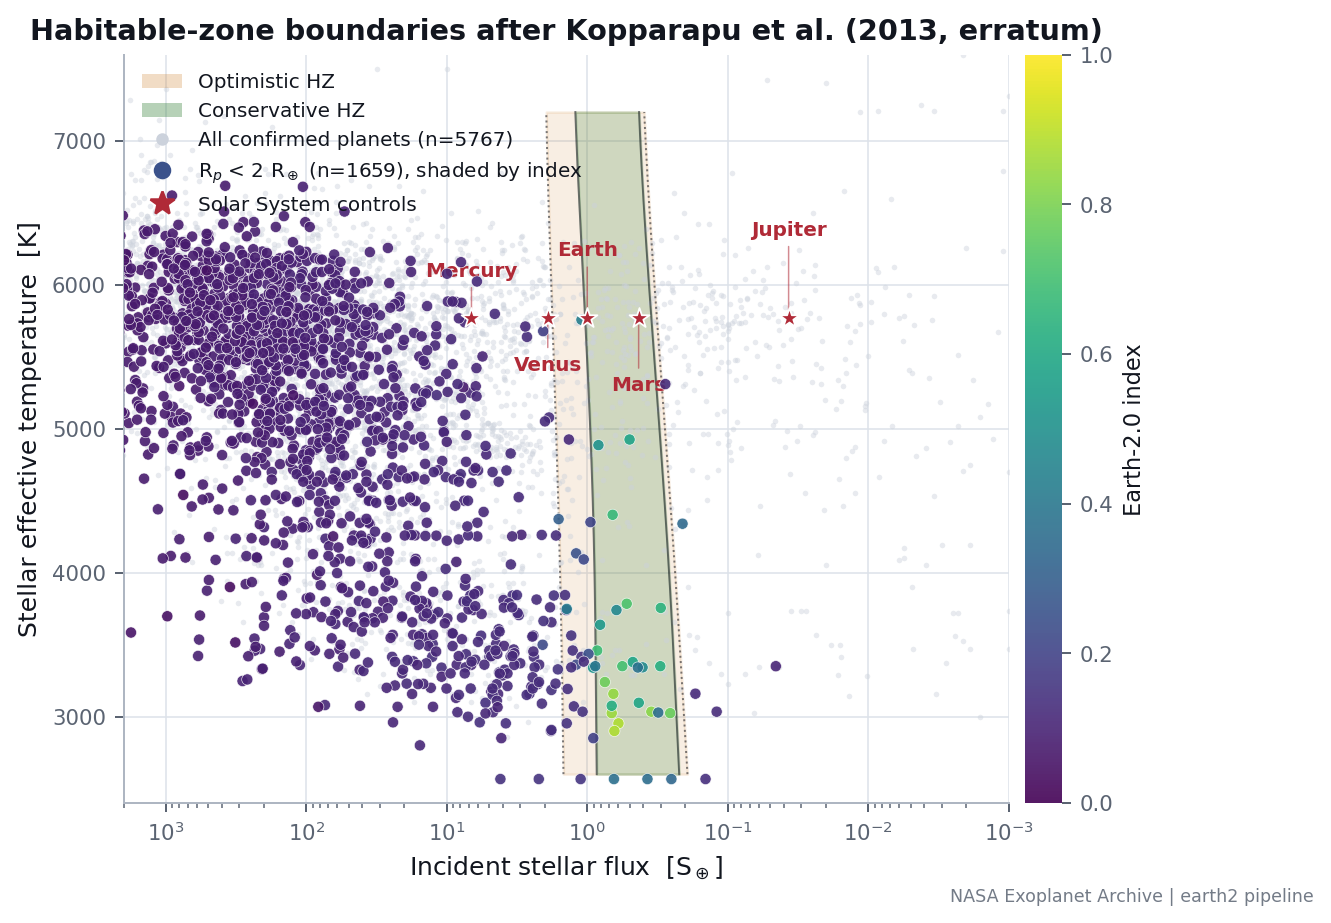
\includegraphics[width=.90\linewidth,height=84mm,keepaspectratio]{finding-earth-2.png}\end{center}
\figcap{The original saved Finding Earth 2.0 plot [2]: 5,767 planets with incident-flux and temperature data; 1,659 have radii below two Earth radii. The similarity index is not a probability of life. Habitable-zone placement alone does not establish surface habitability.}

\subsection*{Observer and target must share a reference frame}
Let $\mathbf r_i$ be a target's position and $\mathbf r_{\mathrm{obs}}$ the observer's position. Their relative position $\mathbf q_i$, distance $D_i$ and sightline $\widehat{\mathbf n}_i$ are
\begin{align}
 \mathbf r_{\mathrm{obs}}(t)&=\mathbf r_\odot(t)+\mathbf r_{\oplus/\odot}(t), &
 \mathbf q_i(t)&=\mathbf r_i(t)-\mathbf r_{\mathrm{obs}}(t),\label{eq:relative}\\
 D_i(t)&=\lVert\mathbf q_i(t)\rVert, &
 \widehat{\mathbf n}_i(t)&=\frac{\mathbf q_i(t)}{D_i(t)}.
\end{align}
For a sufficiently short interval,
\begin{equation}
 \Delta\theta_i\simeq\frac{\lVert\mathbf v_{i,\mathrm{rel},\perp}\rVert\,\Delta t}{D_i}.
\end{equation}
A transverse \emph{relative} speed of $30\unit{km\,s^{-1}}$ at $100\unit{ly}$ gives about $20.6$ arcseconds in 100 years. The Sun's total Galactic speed cannot be substituted for this relative transverse velocity.

\subsection*{A changed sightline is not automatically a new detection}
For a circular orbit, transit geometry depends on the orbital inclination $i$ to the sightline:
\begin{equation}
 b(t)=\frac{a\cos i(t)}{R_\star},\qquad
 |b|<1+\frac{R_p}{R_\star},\qquad
 P_{\mathrm{transit}}\simeq\frac{R_\star+R_p}{a}.
\end{equation}
Here $b$ is the impact parameter, $a$ the orbital radius, and $R_\star,R_p$ the stellar and planetary radii. An Earth--Sun analogue has an isotropic transit probability near $0.47\%$. Changing the view can open \emph{or close} a transit window; detection also requires adequate signal, cadence and orbital phase. Time-dependent Earth-transit-zone membership is already established research [3].
